\begin{enumerate}[label=\thesection.\arabic*,ref=\thesection.\theenumi]
\item A charged particle oscillates about its mean equilibrium position with a frequency of $10^9Hz$. What is the frequency of the electromagnetic waves produced by the oscillator? \\
\solution
\iffalse
\let\negmedspace\undefined
\let\negthickspace\undefined
\documentclass[journal,12pt,twocolumn]{IEEEtran}
\usepackage{cite}
\usepackage{amsmath,amssymb,amsfonts,amsthm}
\usepackage{algorithmic}
\usepackage{graphicx}
\usepackage{textcomp}
\usepackage{xcolor}
\usepackage{txfonts}
\usepackage{listings}
\usepackage{enumitem}
\usepackage{mathtools}
\usepackage{gensymb}
\usepackage{comment}
\usepackage[breaklinks=true]{hyperref}
\usepackage{tkz-euclide} 
\usepackage{listings}
\usepackage{gvv}                                        
\def\inputGnumericTable{}                                 
\usepackage[latin1]{inputenc}                                
\usepackage{color}                                            
\usepackage{array}                                            
\usepackage{longtable}                                       
\usepackage{calc}                                             
\usepackage{multirow}                                         
\usepackage{hhline}                                           
\usepackage{ifthen}                                           
\usepackage{lscape}
\usepackage[export]{adjustbox}

\newtheorem{theorem}{Theorem}[section]
\newtheorem{problem}{Problem}
\newtheorem{proposition}{Proposition}[section]
\newtheorem{lemma}{Lemma}[section]
\newtheorem{corollary}[theorem]{Corollary}
\newtheorem{example}{Example}[section]
\newtheorem{definition}[problem]{Definition}
\newcommand{\BEQA}{\begin{eqnarray}}
\newcommand{\EEQA}{\end{eqnarray}}
\newcommand{\define}{\stackrel{\triangle}{=}}
\theoremstyle{remark}
\newtheorem{rem}{Remark}
\begin{document}
\parindent 0px
\bibliographystyle{IEEEtran}

\title{Assignment\\[1ex]12.8 - 6}
\author{EE23BTECH11034 - Prabhat Kukunuri$^{}$% <-this % stops a space
}
\maketitle
\newpage
\bigskip

\renewcommand{\thefigure}{\theenumi}
\renewcommand{\thetable}{\theenumi}
\section*{Question}
A charged particle oscillates about its mean equilibrium position with a frequency of $10^9Hz$. What is the frequency of the electromagnetic waves produced by the oscillator?

\section*{Solution}
\fi
\begin{table}[h]
    \centering
    \begin{tabular}{|c|c|c|}
    \hline
   Symbol&Value&Description\\ \hline
   $y(t)$&$\cos\brak{2{\pi}f_ct}$&Wave equation of electro-magnetic wave\\ \hline
   $f_c$&$10^9$&Frequency of electromagnetic wave\\ \hline
   $t$&seconds&Time\\ \hline

    \end{tabular}
    \caption{Variable description}
    \label{tab:12.8.6.1}
\end{table}

\begin{figure}[h]
    \centering
    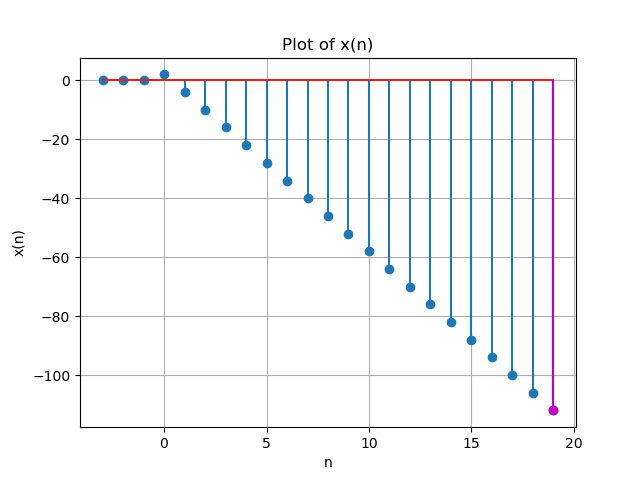
\includegraphics[width=\columnwidth]{Figure_1.png}
    \caption{$y(t)=\cos\brak{2{\pi}\times 10^9t}$}
    \label{fig:12.8.6.2}
\end{figure}
%\end{document}
\pagebreak
Given below are some functions of x and t to 
represent the displacement (transverse
or longitudinal) of an elastic wave. State which of these represents \brak i travelling
wave, \brak {ii} a stationary wave or \brak {iii} none at all: \\
\begin{enumerate}
\item $y = 2\cos \brak{3x} \sin \brak{10t}$
\item $y=2\sqrt{x-vt}$
\item $y = 3\sin \brak{5x - 0.5t} + 4\cos \brak{5x - 0.5t}$
\item $y = \cos x \sin t + \cos 2x \sin 2t$
\end{enumerate}
\solution
\iffalse
\let\negmedspace\undefined
\let\negthickspace\undefined
\documentclass[journal,12pt,twocolumn]{IEEEtran}
\usepackage{cite}
\usepackage{amsmath,amssymb,amsfonts,amsthm}
\usepackage{algorithmic}
\usepackage{graphicx}
\usepackage{textcomp}
\usepackage{xcolor}
\usepackage{txfonts}
\usepackage{listings}
\usepackage{enumitem}
\usepackage{mathtools}
\usepackage{gensymb}
\usepackage{comment}
\usepackage[breaklinks=true]{hyperref}
\usepackage{tkz-euclide} 
\usepackage{listings}
\usepackage{gvv}                                        
\def\inputGnumericTable{}                                 
\usepackage[latin1]{inputenc}                                
\usepackage{color}                                            
\usepackage{array}                                            
\usepackage{longtable}                                       
\usepackage{calc}                                             
\usepackage{multirow}                                         
\usepackage{hhline}                                           
\usepackage{ifthen}                                           
\usepackage{lscape}
\newtheorem{theorem}{Theorem}[section]
\newtheorem{problem}{Problem}
\newtheorem{proposition}{Proposition}[section]
\newtheorem{lemma}{Lemma}[section]
\newtheorem{corollary}[theorem]{Corollary}
\newtheorem{example}{Example}[section]
\newtheorem{definition}[problem]{Definition}
\newcommand{\BEQA}{\begin{eqnarray}}
\newcommand{\EEQA}{\end{eqnarray}}
\newcommand{\define}{\stackrel{\triangle}{=}}
\theoremstyle{remark}
\newtheorem{rem}{Remark}
\begin{document}
\parindent 0px
\bibliographystyle{IEEEtran}
\title{ASSIGNMENT11.15\_13Q}
\author{EE22BTECH11219 - Sai Sujan Rada$^{}$% <-this % stops a space
}
\maketitle
\newpage
\bigskip
\section*{QUESTION}
Given below are some functions of x and t to 
represent the displacement (transverse
or longitudinal) of an elastic wave. State which of these represents \brak i travelling
wave, \brak {ii} a stationary wave or \brak {iii} none at all: \\
\begin{enumerate}
\item $y = 2\cos \brak{3x} \sin \brak{10t}$
\item $y=2\sqrt{x-vt}$
\item $y = 3\sin \brak{5x - 0.5t} + 4\cos \brak{5x - 0.5t}$
\item $y = \cos x \sin t + \cos 2x \sin 2t$
\end{enumerate}
\solution 

\fi
\begin{table}[htbp]
    \centering
    \def\arraystretch{1.5}
    \begin{tabular}{|p{4cm}|p{4cm}|}
    \hline
TRAVELLING WAVE  & STATIONARY WAVE \\ \hline
    $y \brak{x,t} =A \sin  \brak{kx \pm \omega t} $ & $y\brak{ x,t }=A\sin kx\cos \omega t $ \\   \hline
    \hline
PARAMETERS  & DEFINITION  \\  \hline
$A$    &  Amplitude  \\ \hline
 $\omega$  & Angular Velocity  \\  \hline
 $x$    & Position  \\  \hline
 $k$    & Wavenumber    \\  \hline 
    \end{tabular}
    \caption{Travelling wave $vs$ Stationary wave}
    \label{tab:table11.15.13.1}
\end{table}

Let us assume an equation:
\begin{align}
y=A(x)\cos \brak{\omega t+\phi\brak {x}}
\end{align}
\begin{table}[htbp]
    \centering
    \def\arraystretch{1.5}
    \begin{tabular}{|p{4cm}|p{4cm}|}
    \hline
STATIONARY WAVE CONDITION & TRAVELLING WAVE CONDITION \\ \hline
        \brak 1 $A(x)$ should be a function of position x, and it can be expressed as $A(x)=A_{0}cos(\omega t+\alpha)$ where $A_{0}$ is a constant, $k$ is the wavenumber, $x$ is the position and $\alpha$ is a phase constant. & 
        \brak 1 $A(x)$ should be a constant, and it can be expressed as $A(x)=A_{0}$ where $A_{0}$ is a constant number. \\ \hline

        \brak 2 $\phi (x)$ can be expressed as $\phi (x)=c$ where c is a constant. &
        \brak 2 $\phi (x)$ represents a linear expression in x, and it can be expressed as $\phi (x)=kx+\theta$ where k is the wavenumber and $\theta$ is the phaseconstant. \\ \hline
\end{tabular}
    \caption{Travelling wave $vs$ Stationary wave}
    \label{tab:table1}
\end{table}

\begin{figure}[ht]
                        \centering
                        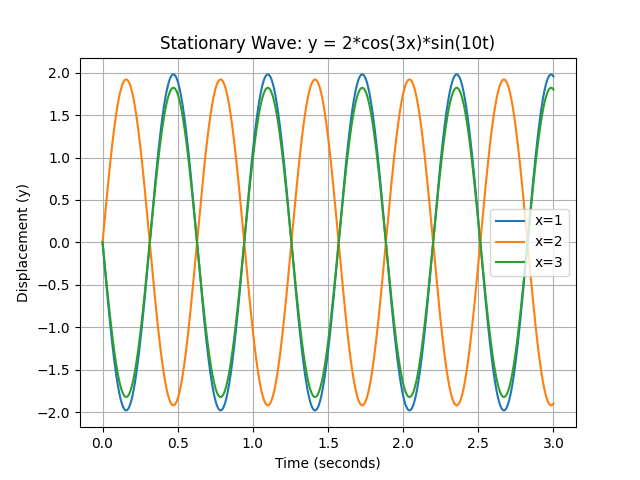
\includegraphics[width=\columnwidth]{figs/a.png}
                        \caption{DIPLACEMENT $vs$ TIME-graph1}
                        \label{fig:11.15.13.1}
\end{figure}
\begin{figure}[ht]
                            \centering
                            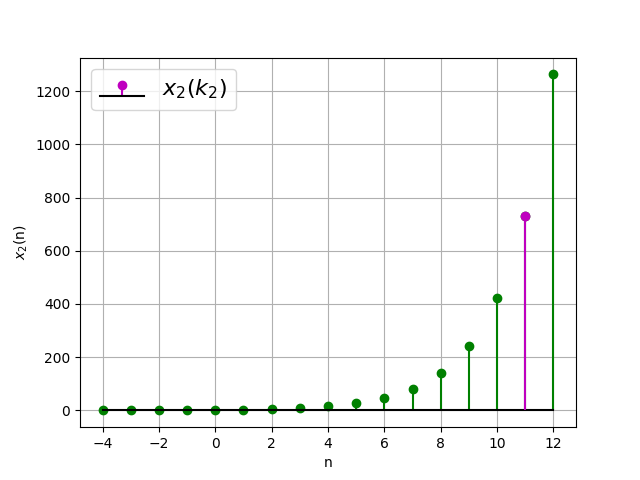
\includegraphics[width=\columnwidth]{figs/b.png}
                            \caption{DIPLACEMENT $vs$ TIME-graph2}
                            \label{fig:11.15.13.2}
\end{figure}   
\begin{figure}[ht]
                             \centering
                             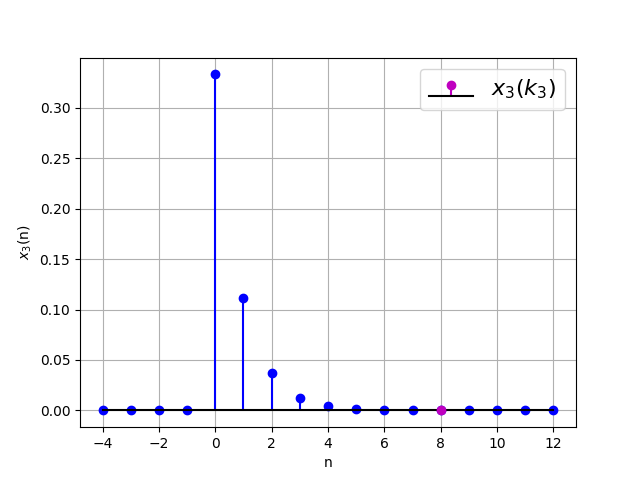
\includegraphics[width=\columnwidth]{figs/c.png}
                             \caption{DIPLACEMENT $vs$ TIME-graph3}
                             \label{fig:11.15.13.3}
\end{figure}
\begin{figure}[ht]
                            \centering
                            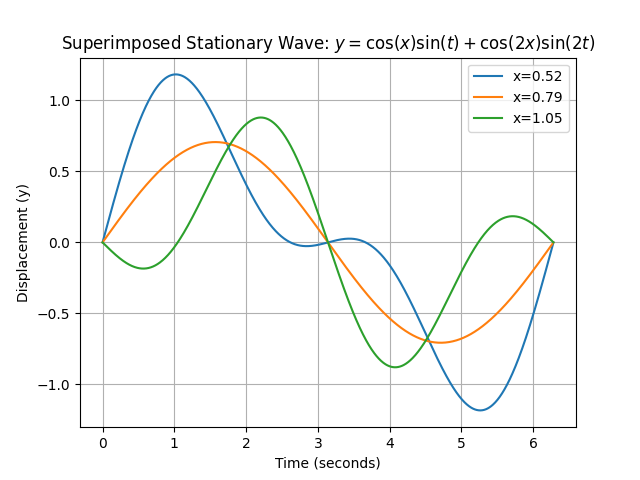
\includegraphics[width=\columnwidth]{figs/d.png}
                            \caption{DIPLACEMENT $vs$ TIME-graph4}
                            \label{fig:11.15.13.4}
\end{figure}
\figref{fig:11.15.13.1} and \figref{fig:11.15.13.3} are self explanatory for stationary and travelling waves.\figref{fig:11.15.13.2} and \figref{fig:11.15.13.4} are neither stationary nor travelling waves.


\pagebreak
\item For the travelling harmonic wave
$y\brak {x, t} = 2.0 \cos 2\pi \brak{10t - 0.0080 x + 0.35}$ where $x$ and $y$ are in $cm$ and $t$ in $s$. Calculate the phase difference between oscillatory
motion of two points separated by a distance of 

\begin{enumerate} [label=(\alph*)]
    \item $4 m$
    \item $0.5 m$
    \item $\lambda/2$
    \item $3\lambda/4$
\end{enumerate}
\solution
% \iffalse
\let\negmedspace\undefined
\let\negthickspace\undefined
\documentclass[journal,12pt,twocolumn]{IEEEtran}
\usepackage{cite}
\usepackage{amsmath,amssymb,amsfonts,amsthm}
\usepackage{algorithmic}
\usepackage{graphicx}
\usepackage{textcomp}
\usepackage{xcolor}
\usepackage{txfonts}
\usepackage{listings}
\usepackage{enumitem}
\usepackage{mathtools}
\usepackage{gensymb}
\usepackage{comment}
\usepackage[breaklinks=true]{hyperref}
\usepackage{tkz-euclide} 
\usepackage{listings}
\usepackage{gvv}                                        
\def\inputGnumericTable{}                                 
\usepackage[latin1]{inputenc}                               \usepackage{caption}
\usepackage{color}                                            
\usepackage{array}                                            
\usepackage{longtable}                                       
\usepackage{calc}                                             
\usepackage{multirow}                                         
\usepackage{hhline}                                           
\usepackage{ifthen}                                           
\usepackage{lscape}

\newtheorem{theorem}{Theorem}[section]
\newtheorem{problem}{Problem}
\newtheorem{proposition}{Proposition}[section]
\newtheorem{lemma}{Lemma}[section]
\newtheorem{corollary}[theorem]{Corollary}
\newtheorem{example}{Example}[section]
\newtheorem{definition}[problem]{Definition}
\newcommand{\BEQA}{\begin{eqnarray}}
\newcommand{\EEQA}{\end{eqnarray}}
\newcommand{\define}{\stackrel{\triangle}{=}}
\theoremstyle{remark}
\newtheorem{rem}{Remark}
\begin{document}

\bibliographystyle{IEEEtran}
\vspace{3cm}

\title{NCERT 11.15. Q10}
\author{EE23BTECH11010 - Venkatesh Bandawar$^{*}$% <-this % stops a space
}
\maketitle
\newpage
\bigskip

\renewcommand{\thefigure}{\arabic{figure}}
\renewcommand{\thetable}{\arabic{table}}

\bibliographystyle{IEEEtran}

\parindent 0px
\textbf{Question:} For the travelling harmonic wave
$y\brak {x, t} = 2.0 \cos 2\pi \brak{10t - 0.0080 x + 0.35}$ where $x$ and $y$ are in $cm$ and $t$ in $s$. Calculate the phase difference between oscillatory
motion of two points separated by a distance of 

\begin{enumerate} [label=(\alph*)]
    \item $4 m$
    \item $0.5 m$
    \item $\lambda/2$
    \item $3\lambda/4$
\end{enumerate}

\textbf{Solution:}  
\begin{table}[htbp] \small
\centering
\begin{table}[ht]
    \centering
    \begin{tabular}{|c|c|c|}
        \hline
        Parameter & Value & Description \\
        \hline
        $x(0)$ & 5 & First term of AP \\
        $d$ & 1.75 & Common difference of AP \\
        $x(n)$ & 20.75 & $n^{th}$ term of AP \\
        \hline
    \end{tabular}
    \vspace{2mm}
    \caption{Parameter List}
    \label{tab:simple.10.5.2.20}
\end{table}

\caption{Given \, parameters list}
\label{tab:given parameters list}
\end{table}
\begin{align}
    \brak{\Delta \theta} &= \brak{ 2\pi f t - kx_1 + \phi}  - \brak{2\pi f t -kx_2 + \phi}\\
    &= k\brak{x_2 - x_1} 
\end{align}

\begin{table}[htbp] 
\centering
\begin{tabular}{|c|c|c|}
        \hline
        \textbf{Parameter} & \textbf{Value} & \textbf{Description} \\
        \hline
        $x(0)$ & & First term \\
        \hline
        $r$ & & Common ratio \\
        \hline
        $x(0)^3r^3$ & 1 & Product of terms \\
        \hline
        $x(0)$ + $x(0)r$ + $x(0)r^2$ & $\frac{39}{10}$ & Sum of terms \\
        \hline
    \end{tabular}

\caption{Phase \, differences}
\label{tab:phase differences}
\end{table}

\begin{figure}[!h] 
\centering
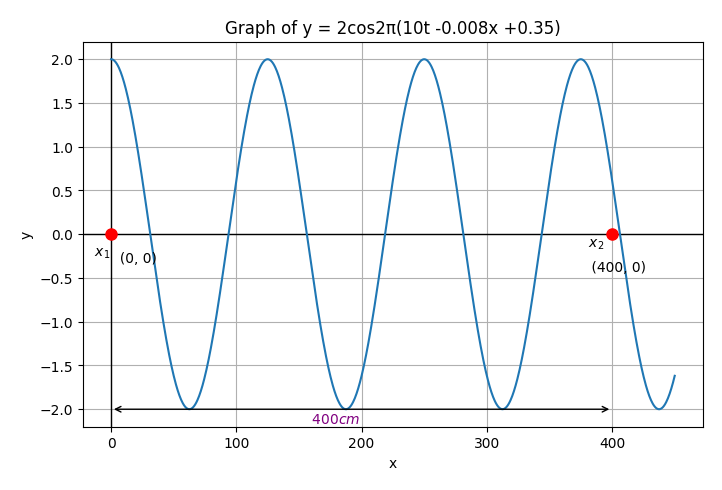
\includegraphics[width=\columnwidth]{figs/graph1.png}
\captionsetup{justification=centering}
\caption{}
\label{fig:Graph1}
\end{figure}

\begin{figure}[!h] 
\centering
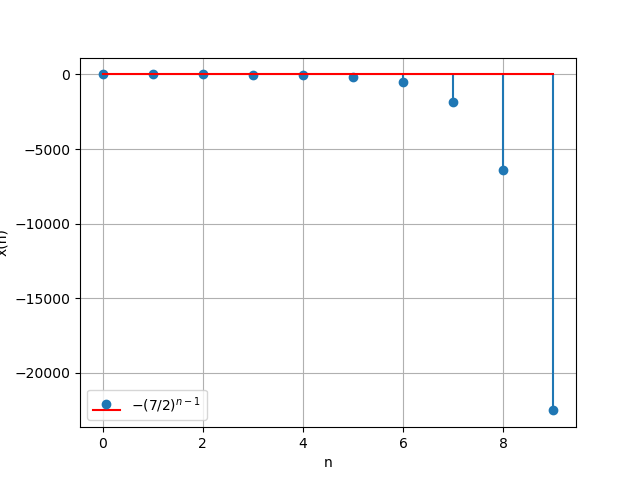
\includegraphics[width=\columnwidth]{figs/graph2.png}
\captionsetup{justification=centering}
\caption{}
\label{fig:Graph2}
\end{figure}

\begin{figure}[!h] 
\centering
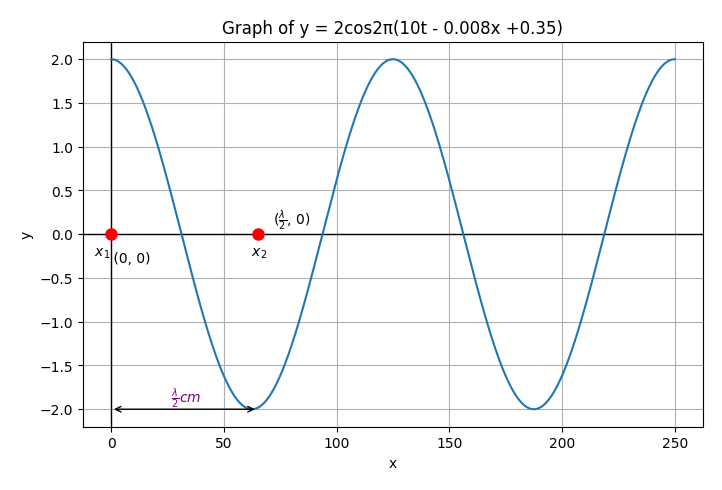
\includegraphics[width=\columnwidth]{figs/graph3.png}
\captionsetup{justification=centering}
\caption{}
\label{fig:Graph3}
\end{figure}

\begin{figure}[!h] 
\centering
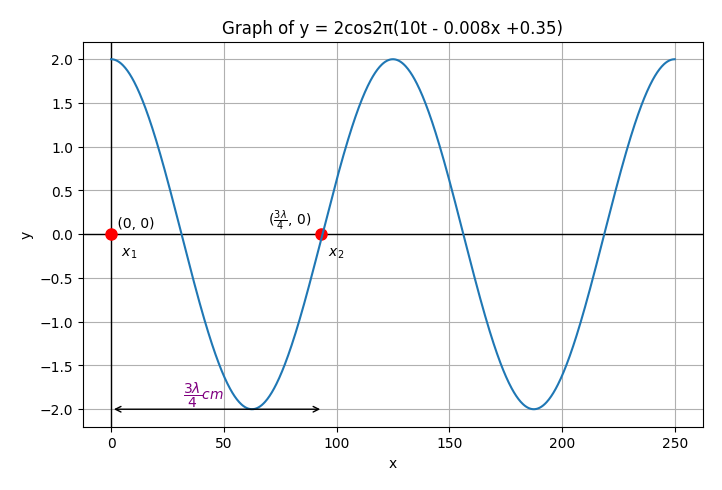
\includegraphics[width=\columnwidth]{figs/graph4.png}
\captionsetup{justification=centering}
\caption{}
\label{fig:Graph4}
\end{figure}



\end{document}


\pagebreak
Suppose that the electric field amplitude of an electromagnetic wave is $E_0$ = 120N/C and that its frequency is $f$ = 50.0 MHz.\\
\begin{enumerate} [label=(\alph*)]
    \item Determine, $B_0, \omega, k$ and $\lambda$
    \item Find expressions for \textbf{E} and \textbf{B}
\end{enumerate}
\solution
\iffalse
\let\negmedspace\undefined
\let\negthickspace\undefined
\documentclass[journal,12pt,twocolumn]{IEEEtran}
\usepackage{cite}
\usepackage{amsmath,amssymb,amsfonts,amsthm}
\usepackage{algorithmic}
\usepackage{graphicx}

\usepackage{textcomp}
\usepackage{xcolor}
\usepackage{txfonts}
\usepackage{listings}
\usepackage{enumitem}
\usepackage{mathtools}
\usepackage{gensymb}
\usepackage{comment}
\usepackage[breaklinks=true]{hyperref}
\usepackage{tkz-euclide} 
\usepackage{listings}
\usepackage{gvv}                                                                      
\usepackage[latin1]{inputenc}                                
\usepackage{color}                                            
\usepackage{array}                                            
\usepackage{longtable}                                       
\usepackage{calc}                                             
\usepackage{multirow}                                         
\usepackage{hhline}                                           
\usepackage{ifthen}                                           
\usepackage{lscape}
\setlength{\arrayrulewidth}{0.5mm}
\setlength{\tabcolsep}{18pt}
\renewcommand{\arraystretch}{1.5}
\newtheorem{theorem}{Theorem}[section]
\newtheorem{problem}{Problem}
\newtheorem{proposition}{Proposition}[section]
\newtheorem{lemma}{Lemma}[section]
\newtheorem{corollary}[theorem]{Corollary}
\newtheorem{example}{Example}[section]
\newtheorem{definition}[problem]{Definition}
\newcommand{\BEQA}{\begin{eqnarray}}
\newcommand{\EEQA}{\end{eqnarray}}
\newcommand{\define}{\stackrel{\triangle}{=}}
\theoremstyle{remark}
\newtheorem{rem}{Remark}

\begin{document}

\bibliographystyle{IEEEtran}
\vspace{3cm}

\title{NCERT 12.8 8}
\author{EE23BTECH11054 - Sai Krishna Shanigarapu% <-this % stops a space
}
\maketitle
\newpage
\bigskip

\begin{flushleft}
\textbf{Question 8}\\
Suppose that the electric field amplitude of an electromagnetic wave is $E_0$ = 120N/C and that its frequency is $f$ = 50.0 MHz.\\
(a) Determine, $B_0, \omega, k$ and $\lambda$\\
(b) Find expressions for \textbf{E} and \textbf{B}\\
\end{flushleft}

\bigskip


Solution:
\fi

\begin{center}
    \begin{table}[ht]
        \caption{Input Parameters}
        \setlength{\arrayrulewidth}{0.3mm}
\setlength{\tabcolsep}{15pt}
\renewcommand{\arraystretch}{1.5}

%\textbf{Table 1}\\
\begin{center}
\begin{tabular}{ |p{1cm}|p{2.5cm}|p{1.7cm}|  }

\hline
Symbol& Description&value\\
\hline
$f$ & frequency of source & 50.0 MHz\\
\hline
$E_0$ & Electric field amplitude  & 120 N/C\\
\hline
$c$ &speed of light & 3 x 10$^8$ m/s \\
\hline
$\vec{e_2}, \vec{e_3}$ & Standard Basis vectors & N/A\\
\hline

\end{tabular}
\end{center}
        \label{tab:table1.12.8.8}
    \end{table}
\end{center}


\begin{flushleft}
    \begin{table}[ht]
       \caption{Formulae and Output}
       \setlength{\arrayrulewidth}{0.3mm}
\setlength{\tabcolsep}{15pt}
\renewcommand{\arraystretch}{1.5}

%\textbf{Table 1}\\
\begin{center}
\begin{tabular}{ |p{1cm}|p{2.5cm}|p{1.7cm}|  }

\hline
Symbol& Description&value\\
\hline
$f$ & frequency of source & 50.0 MHz\\
\hline
$E_0$ & Electric field amplitude  & 120 N/C\\
\hline
$c$ &speed of light & 3 x 10$^8$ m/s \\
\hline
$\vec{e_2}, \vec{e_3}$ & Standard Basis vectors & N/A\\
\hline

\end{tabular}
\end{center}
       \label{tab:table2.12.8.8}
    \end{table}
\bigskip
\end{flushleft}

\bigskip


\newpage
\renewcommand{\thefigure}{\theenumi}
\renewcommand{\thetable}{\theenumi}

\begin{flushleft}

\begin{figure}[h]
\renewcommand\thefigure{1}
  \caption{Graphs of $\vec{E} \text{ and } \vec{B}$}
  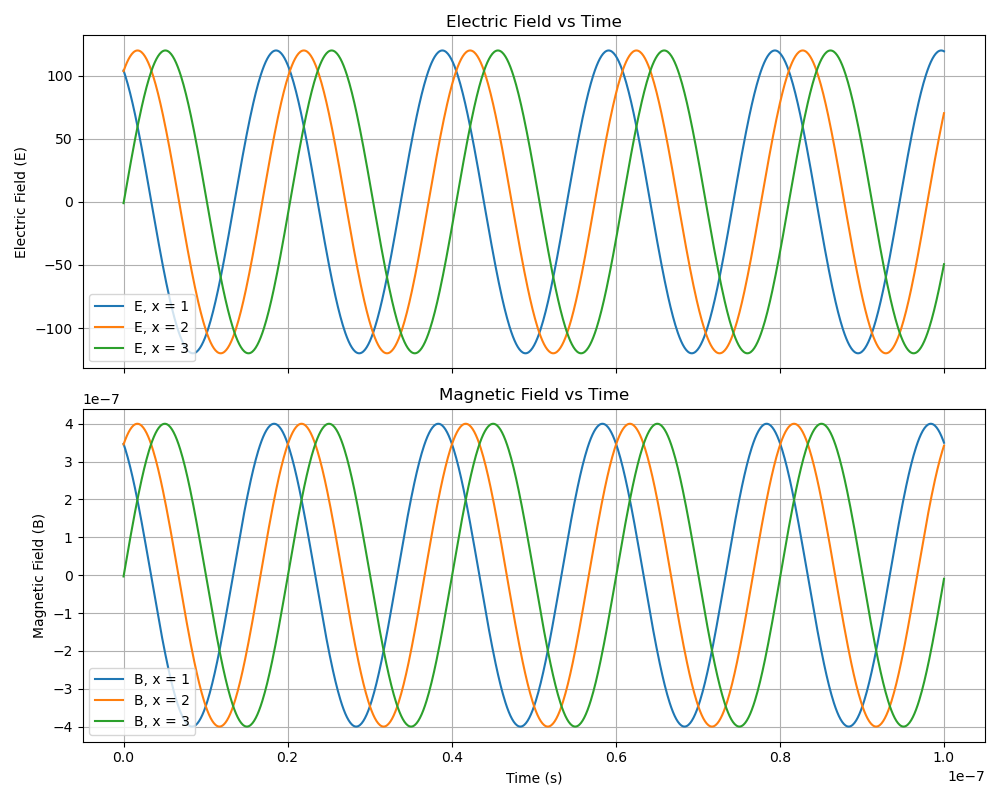
\includegraphics[width=1.05\columnwidth]{ncert-physics/12/8/8/figs/Figure_1.png}
  \label{fig:fig1.12.8.8}

\end{figure}

\end{flushleft}

%\end{document}


\end{enumerate}
